\documentclass[UTF8]{ctexart}

\usepackage{listings}
\usepackage{color,xcolor} 
\usepackage{colortbl}
\usepackage{graphicx}
\usepackage{booktabs} %绘制表格
\usepackage{caption2} %标题居中
\usepackage{geometry}
\usepackage{array}
\usepackage{amsmath}
\usepackage{subfigure} 
\usepackage{longtable}
\usepackage{abstract}
\usepackage{multirow}
\usepackage{enumerate}
\usepackage{float}

\pagestyle{plain} %页眉消失

\geometry{a4paper,left=2.5cm,right=2.5cm,top=2.5cm,bottom=2.5cm}%设置页面尺寸
\lstset{
		numbers=left, %设置行号位置
		numberstyle=\tiny, %设置行号大小	
		keywordstyle=\color{blue}, %设置关键字颜色
		commentstyle=\color[cmyk]{1,0,1,0}, %设置注释颜色
		escapeinside=``, %逃逸字符(1左面的键),用于显示中文
		breaklines, %自动折行
		extendedchars=false, %解决代码跨页时,章节标题,页眉等汉字不显示的问题
		xleftmargin=1em,xrightmargin=1em, aboveskip=1em, %设置边距
		tabsize=4, %设置tab空格数
		showspaces=false %不显示空格
	}


		% \begin{figure}[!htbp]\centering
		% \includegraphics[width=1\textwidth]{img} % 图片相对位置
		% \label{fig:figure 0} % 图片标签
		% \end{figure}




\title{基于\textbf{XXXXX}XX的葡萄酒评价}
\date{August 24, 2022}

\begin{document}
    \maketitle
	\renewcommand{\abstractname}{\Large 摘要\\}
	\begin{abstract}
		\normalsize
% 		自2019年年末新型冠状病毒首次被发现以后,一场新冠肺炎疫情便迅速爆发并蔓延至全球,不但造成了大量的死亡,而且对世界各国政治、经济等多个方面也都产生了重大的影响。时至今日,人类仍然未能彻底战胜疫情。因此,本文将试图根据中国的疫情状况建立数学模型,并以此来预测中国新型冠状肺炎的发展趋势。
		
% 		首先,我们根据中国的疫情数据,利用微分方程,在SIR传染病模型的基础上,充分结合了中国的疫情防控现实状况,对该模型进行了优化修正,从而建立了SIR-YN传染病模型,并由此对中国的疫情发展做出了预测。
% 然后,我们将预测数据与实际数据进行对比,评估了所建立模型的精准度,并分析了误差的产生原因。
% 最后,我们针对误差的产生原因,提出了改进模型的方向,并综合评价了该模型的优缺点。

%         最后得出结果。
		摘要部分...............

		\textbf{关键字}:xxxxxxx
	\end{abstract}

	
	\section{问题背景与重述}
		\subsection{问题背景}
		葡萄酒是当今世界上最畅销的酒类之一,在各种场合都有葡萄酒的身影。然而葡萄酒的酿造是取决于多种因素,各种因素的叠加会导致葡萄酒的品质差异明显。在不同的原材料已经酿制方法的差别下葡萄酒会继续细分,例如红葡萄酒和白葡萄酒等。对各种葡萄酒的鉴别是必不可少的一个步骤,而采用人工品尝打分和采用仪器进行理化指标的检验已成为最为科学的鉴别方法。最后经过安全检查、筛选分级的葡萄酒方可上市成为饮用酒。
		\subsection{题目所给信息及参数}
		此次比赛是根据10位品酒员为27款红酒和28款白葡萄酒的打分,以及上述葡萄酒的指标情况和芳香物质为基础进行数学分析和建模,并探讨品酒员的打分是否合理以及论证是否科学分级。红葡萄酒和白葡萄酒的市场在国际上的价值非常之高,葡萄酒依旧是未来的主力酒类,对此分析依旧存在价值。现在根据三个数据文件,并对三个数据进行分析处理后描述统计,完成数学建模和预测。

		数据一:葡萄酒品尝评分表;数据二:指标总表;数据三:芳香物质。
		\subsection{所需解决的问题}
		\begin{itemize}
			\item [{1)}]{根据附件所提供的两组品酒员对27款红葡萄酒和28款白葡萄酒的打分判断两组结果是否有显著性差异,并判断哪一组的更加可信。 }
			\item [2)]{}
			\item [3)]{分析酿酒葡萄和葡萄酒的理化指标之间是否具有相关性,以及其之间具有什么样的联系。}
			\item [4)]{}
		\end{itemize}



	\section{问题分析}
		针对不同的国家,地区和相对应的医疗水平进行对应的数据指标分析。主要分析感染率,病人接触率,治愈率,以及传染期接触数。
		模型构建还需要考虑到新冠肺炎的无症状感染者这一特殊的情况,根据这些指标进行相轨线分析,合理的进行疫情的分析和未来疫情走向以及各地区、国家的防疫政策研究。
		\subsection{问题一的分析}
		第一,根据附件1中给出两组品酒员的打分情况判断两组的打分是否有显著性差异。对于此问题,分析附件一所提供的数据,
		研究发现两组对红葡萄酒和白葡萄酒的打分情况是两两相互比较和配对,适合于先进行单样本K-S检验判断数据是否符合正态分布,
		再进行两配对样本T检验进行显著性差异判断的办法。

		第二,判断两组品酒员的打分情况哪一组更加可信。对于此问题,分析两组品酒员的打分情况,检验两组中打分的更稳定的一方,
		越稳定的分数即代表品酒员偏好更少,更加可信。提取两组品酒员对于白葡萄酒和红葡萄酒的分数的标准差,根据标准差的大小进行可信性的判断。

		\subsection{问题二的分析}
		\subsection{问题三的分析}
		首先要参照附件所给的数据来进行分析酿酒葡萄和葡萄酒之间的相关性,附件的信息内容过多,需要进行合理的过滤和筛选数据,
		但要尽可能保证其数据的完整性和真实性。我们采取相关性分析,依据相关性皮尔森系数来判断葡萄酒的数据和酿酒葡萄的理化指标之间的相关性显著程度。

		在进行了相关性分析后,可以确定下一些具有显著相关的数据流,要进一步解决其葡萄酒某指标与该些理化指标的关系,
		则要进行其关系的拟合,从而得出实质性的结论来判断酿酒葡萄和葡萄酒之间的关系,以及其关系的可靠性。
		\subsection{问题四的分析}
			

		\section{符号说明}

		\section{模型假设}

% 模型假设部分
% 		\begin{itemize}
%   \item [\bf{1)}]\bf{考虑到目前已处于疫情控制阶段,且人们自我隔离意识较好,不妨设每个病人的有效日接触率为定值}
%   \item [2)]\bf{所有人口都为易感染者,不考虑个别免疫体质}
%   \item [3)]\bf{疑似病例一旦确诊即被隔离,不会再传播给他人}
%   \item [4)]\bf{隔离人群中一旦被确定未感染,则立刻结束隔离,即恢复易感者身份}
%   \item [5)]\bf{在考虑隔离者与未隔离者时将确诊感染者和潜伏期患者都定义为感染者}
  
		% \end{itemize}	

% 	\section{符号说明}

		
% 		\begin{table}[!htbp] 
% 		\begin{center}  
% 		\begin{tabular}{c|l}    
% 		\toprule[2pt]    
% 		\rowcolor[gray]{0.8}
		
% 		\multicolumn{1}{m{8em}}{\centering 符号}	&\multicolumn{1}{m{30em}}{\centering 基本说明}\\
		
% 		%直接用合并单元格的方法来实现自定义列宽的同时,使文字居中对齐
		
% 		\midrule[1.3pt]
% 		$S(t)$ & 表示t时刻\ 易感人群\ 的总人数 \\   
% %		$E(t)$ & 表示t时刻\ 潜伏期人数\ 占总人数的比例 \\   
% 		$I(t)$ & 表示t时刻\ 感染人数\ 的总人数\\    
% 		$R(t)$ & 表示t时刻\ 退出者(治愈+死亡)的总人数 \\ 
% 		$Y(t)$ & 表示t时刻\ 疑似者(实际被感染+实际未被感染)的总人数\\    
% 		$N(t)$ & 表示t时刻\ 所有未隔离患者\ 的总人数\\ 
% 		$\kappa$ & 疑似人群中被确定未感染人数占疑似人群总数的比例\\
% 		$\lambda$ &隔离者被确诊人数占隔离者总人数的比例\\
% 		$\theta$ & 被隔离的人数占未隔离总人数的比例\\
% 		$\omega$ & 被确诊且隔离人数占未隔离总人数的比例\\	
% 		$\rho$ &  感染者平均每天对任何状态的人的接触率\\
% 		$\xi$ &  退出率(死亡率+治愈率)\\	
% 		\bottomrule[2pt]   
% 		\end{tabular}  
% 		\end{center}
% 		\end{table}
		
		
% 	\section{问题假设}
% \vspace{4pt}
% \begin{enumerate}[1)]
    % \item  根据已有数据建立预测模型,根据传染病的基本过程,确定了影响疫情变化趋势的各个参量,基于微分方程模型进行未来疫情发展趋势的求解。

    % \item  将预测数据与实际数据进行比对,利用统计学方法进行模型精确度分析,并结合实际情况进行误差来源的分析从而改进所建立的模型。

    % \item  根据已经建立的模型,寻求对疫情发展影响较大的参量,并分析如何改变这些参量来控制疫情,从而提出切实的建议。
% \end{enumerate}  



	\section{模型建立与求解}
		\subsection{问题一的求解}
		问题一分析两组评酒员的评价结果有无显著性差异,并判断两组结果哪一组更加可信。采用三个步骤完成分析,步骤如下:
		\begin{itemize}
			\item [{1)}]{判断数据是否符合正态分布,以选择合适模型;}
			\item [2)]{使用两配对T检验方法完成显著性检验的判断;}
			\item [3)]{计算标准差的大小后进行比较,较小的表示稳定性更高,更加可信。}
	
		\end{itemize}
		
		\subsubsection{数据的预处理}
			因为数据较大,指标较多,所以我们对各项分数相加得到总分,接着取平均值进行比较。

			均值计算如下:
			\begin{equation}
				x = \sum_{x_{mn}}^{10}(m = 1,2,3,,,10  n = 1,2,3,,,10)
			\end{equation}

		\subsubsection{各葡萄酒样本评分数据概率分布的确定}
		对两组品酒员差异性评价的假设检验一般要求数据符合正态分布,因为两配对样本T检验的前提要求为数据符合正态分布,才可以使用T检验的数学模型。 
		利用 SPSS 统计软件中单样本 K-S 检验, 对数据集两组品酒员分别对红、白葡萄酒品尝得到的四组评价结果进行了正态分布检验。

		从图1和图 2可以看出两组的双边检验结果。因此可以认为品酒员对葡萄酒的评分服从正态分布。

		\subsubsection{两组评价结果的显著性差异评价}
		上述检验显示各类葡萄酒得分情况属于正态总体,为了进一步说明品酒员评分的科学性以及两个评分组评分的可信度, 需要检查两组给出的评分是否有显著性差异, 即对数据进行显著性检验。

		两配对样本非参数检验一般用于同一研究对象分别给予两种不同处理的效果比较。因为两组品酒员分别对同一样本组进行评分,故两组数据为配对数据。
		
		\begin{equation}
			z_{li} = w_{li}-w_{2i}(i=1,2,,,,n)
		\end{equation}

		$z_li$来自正态分布,用假设检验的方法,假设$H_{0}:u_1=0$成立;
		\[\left\{\begin{array}{llcl}
				
					\bar{z}=\frac{1}{n}\sum_{i=1}^n(Z_li)\\
				
					s_{1}^2=\frac{1}{n-1}\sum_{i=1}^n(z_li-z_1)^2\\
				
					t=\frac{\bar{z_1}}{\frac{s_1}{\sqrt{n}}}\\
				
					w={\mid t \mid \ge t_{1-\frac{a}{2}}(n-1)}\\
				
				
			
			
		% 	% S(t_0)&=&140005\times10^4&\text{人},\\
		% 	% I(t_0)&=&14052 &\text{人},\\
		% 	% R(t_0)&=&130 &\text{人},\\
		% 	% Y(t_0)&=&4562 &\text{人},\\
		% 	% N(t_0)&=&6336 &\text{人},\\

	\end{array} \right.\]

		对于统计量t,在给定显著性水平a下,该检验问题的拒绝域是w,若{\mid t \mid \ge t_{1-\frac{a}{2}}(n-1)},则拒绝假设反之则接受。

		\begin{center}
			\begin{tabular}{||c c c c c c||} 
			\hline
			组数 & 样本数 & 平均值 & 标准差 &$T_1$值 &p \\ [0.5ex] 
			\hline
			一 & 27 & 73.056 & 3.9780 & 2.458 & 0.0104\\ 
			\hline
			二 & 27 & 70.515 & 7.3426 & 2.458 & 0.0104 \\
			\hline
		   \end{tabular}
		   \end{center}

		   上表给出了两组红葡萄酒评分均值的t检验结果,通过查表当x =0.05, n=27时, $t_{1-\frac{a}{2}}(n-1)=2.0555<2.491$
		   且方差齐性检验的$p$值为0.0104<0.05,
		   所以拒绝原假设,对于红葡萄酒的评价,两组评酒员的评价结果有显著性差异。
		   因为第二组评酒员对红葡萄酒样品评分的标准差大于第一组的,第二组各评酒员得评分差异小,稳定性高,比较可信。

		   对于白葡萄酒采用同样的方法,得到了如下的表格:
		   \begin{center}
			\begin{tabular}{||c c c c c c||} 
			\hline
			组数 & 样本数 & 平均值 & 标准差 &$T_1$值 &p \\ [0.5ex] 
			\hline
			一 & 28 & 74.261 & 5.2012 & -2.184 & 0.01892\\ 
			\hline
			二 & 28 & 76.532 & 3.1709 & -2.184 & 0.01892 \\
			\hline
		   \end{tabular}
		   \end{center}

		   上表给出了两组红葡萄酒评分均值的$t$检验结果,通过查表当$x=0.05$, $n=28$时, $t_{1-\frac{a}{2}}(n-1)=2.0555<2.491$
		   且方差齐性检验的$p$值为0. 01892<0.05,
		   所以拒绝原假设,对于白葡萄酒的评价,两组评酒员的评价结果有显著性差异。因为第一组评酒员对红葡萄酒样品评分的标准差大于第二组,
		   第二组各评酒员得评分差异小,稳定性高,比较可信。

		   综上分别对两组葡萄酒进行t检验,在显著性水平为0.05时,得出两组评酒员的评价结果有显著性差异,第二组评酒员的评分更可信。
		   
		   \subsection{问题二的求解}
		   \subsection{问题三的求解}
		   \subsubsection{数据筛选}
		   所给出酿酒葡萄和葡萄酒的数据十分多,但不能保证没一项指标都有一项对应的指标与他有着显著的相关性,所以需要进行数据指标的筛选,
		   使得其相关性分析,更加可信。在本问中,抽选葡萄酒的花色苷、DPPH半抑制体积、酒总黄酮、色泽这几项数据来进行数据相关性分析。

		   \subsection{相关性分析}
		   相关分析是描述两个变量间关系的密切程度,由相关系数和显著性程度值表示,当相关系数的绝对值越接近于1,则表示两个变量间的相关性越显著,
		   或者显著性*p<0.05,**p<0.01具有上述的效果。
		   双变量系数测量的主要指标有卡方类测量、Spearman相关系数、pearson相关系数等,由于酿酒葡萄和葡萄酒的数据为定距数据,
		   则在进行两者间的相关性检验时用pearson相关系数来判断,其公式为:

		   \begin{equation}
				r=\frac{\sum(x_i-\bar{x})}{\sqrt{\sum(x_i-\bar{x})^2 \sum(y_i-\bar{y})^2}}
		   \end{equation}
		   
		   相关系数r的取值范围为:-1\le r \le 1

		   \[\left\{\begin{array}{llcl}
				r>0为正相关,r<0为负相关\\

				\mid r \mid =0表示不存在线性关系\\

				\mid r \mid =1表示完全线性相关\\

		   \end{array} \right.\]

		   其中皮尔森简单相关系数检验统计为:

		   \begin{equation}
				t=\frac{r sqrt{n-1}}{\sqrt{1-r^2}}
		   \end{equation}

		   其中的t服从n-2个自由度的t分布

		   \subsubsection{相关性检验}
		   通过将筛选出的数据通过spss来进行相关性的检验分析,来发现针对某些特定的葡萄酒指标,有的酿酒葡萄在某个理化指标较为突出的情况下,
		   可以根据需求来进行指定行的处理来满足要求。如下将一次选取花色苷、DPPH半抑制体积、酒总黄酮、色泽这几项数据来进行数据相关性分析。
		   通过对数据进行平均值和标准差统计,成对排除个案缺失值,采用pearson相关系数的双侧显著性检验来获取结果。如下为结果图。
		
		   

			% 通过观察数据表的pearson相关性数据可以发现葡萄酒中花色苷的指标与褐变度、苹果酸、单宁、果梗比等数据的相关性较为显著,从而可以知道
			% 该些酿酒葡萄的理化指标对花色苷的影响较为明显,同时也通过该表可以得出一些负相关的理化指标。
			
			% 同理进行DPPH半抑制体积、酒总黄酮、色泽其余三项数据的分析,分别得出相关性分析结果

			% 如图为DPPH半抑制体积的相关性分析
				\begin{figure}[H]\centering
				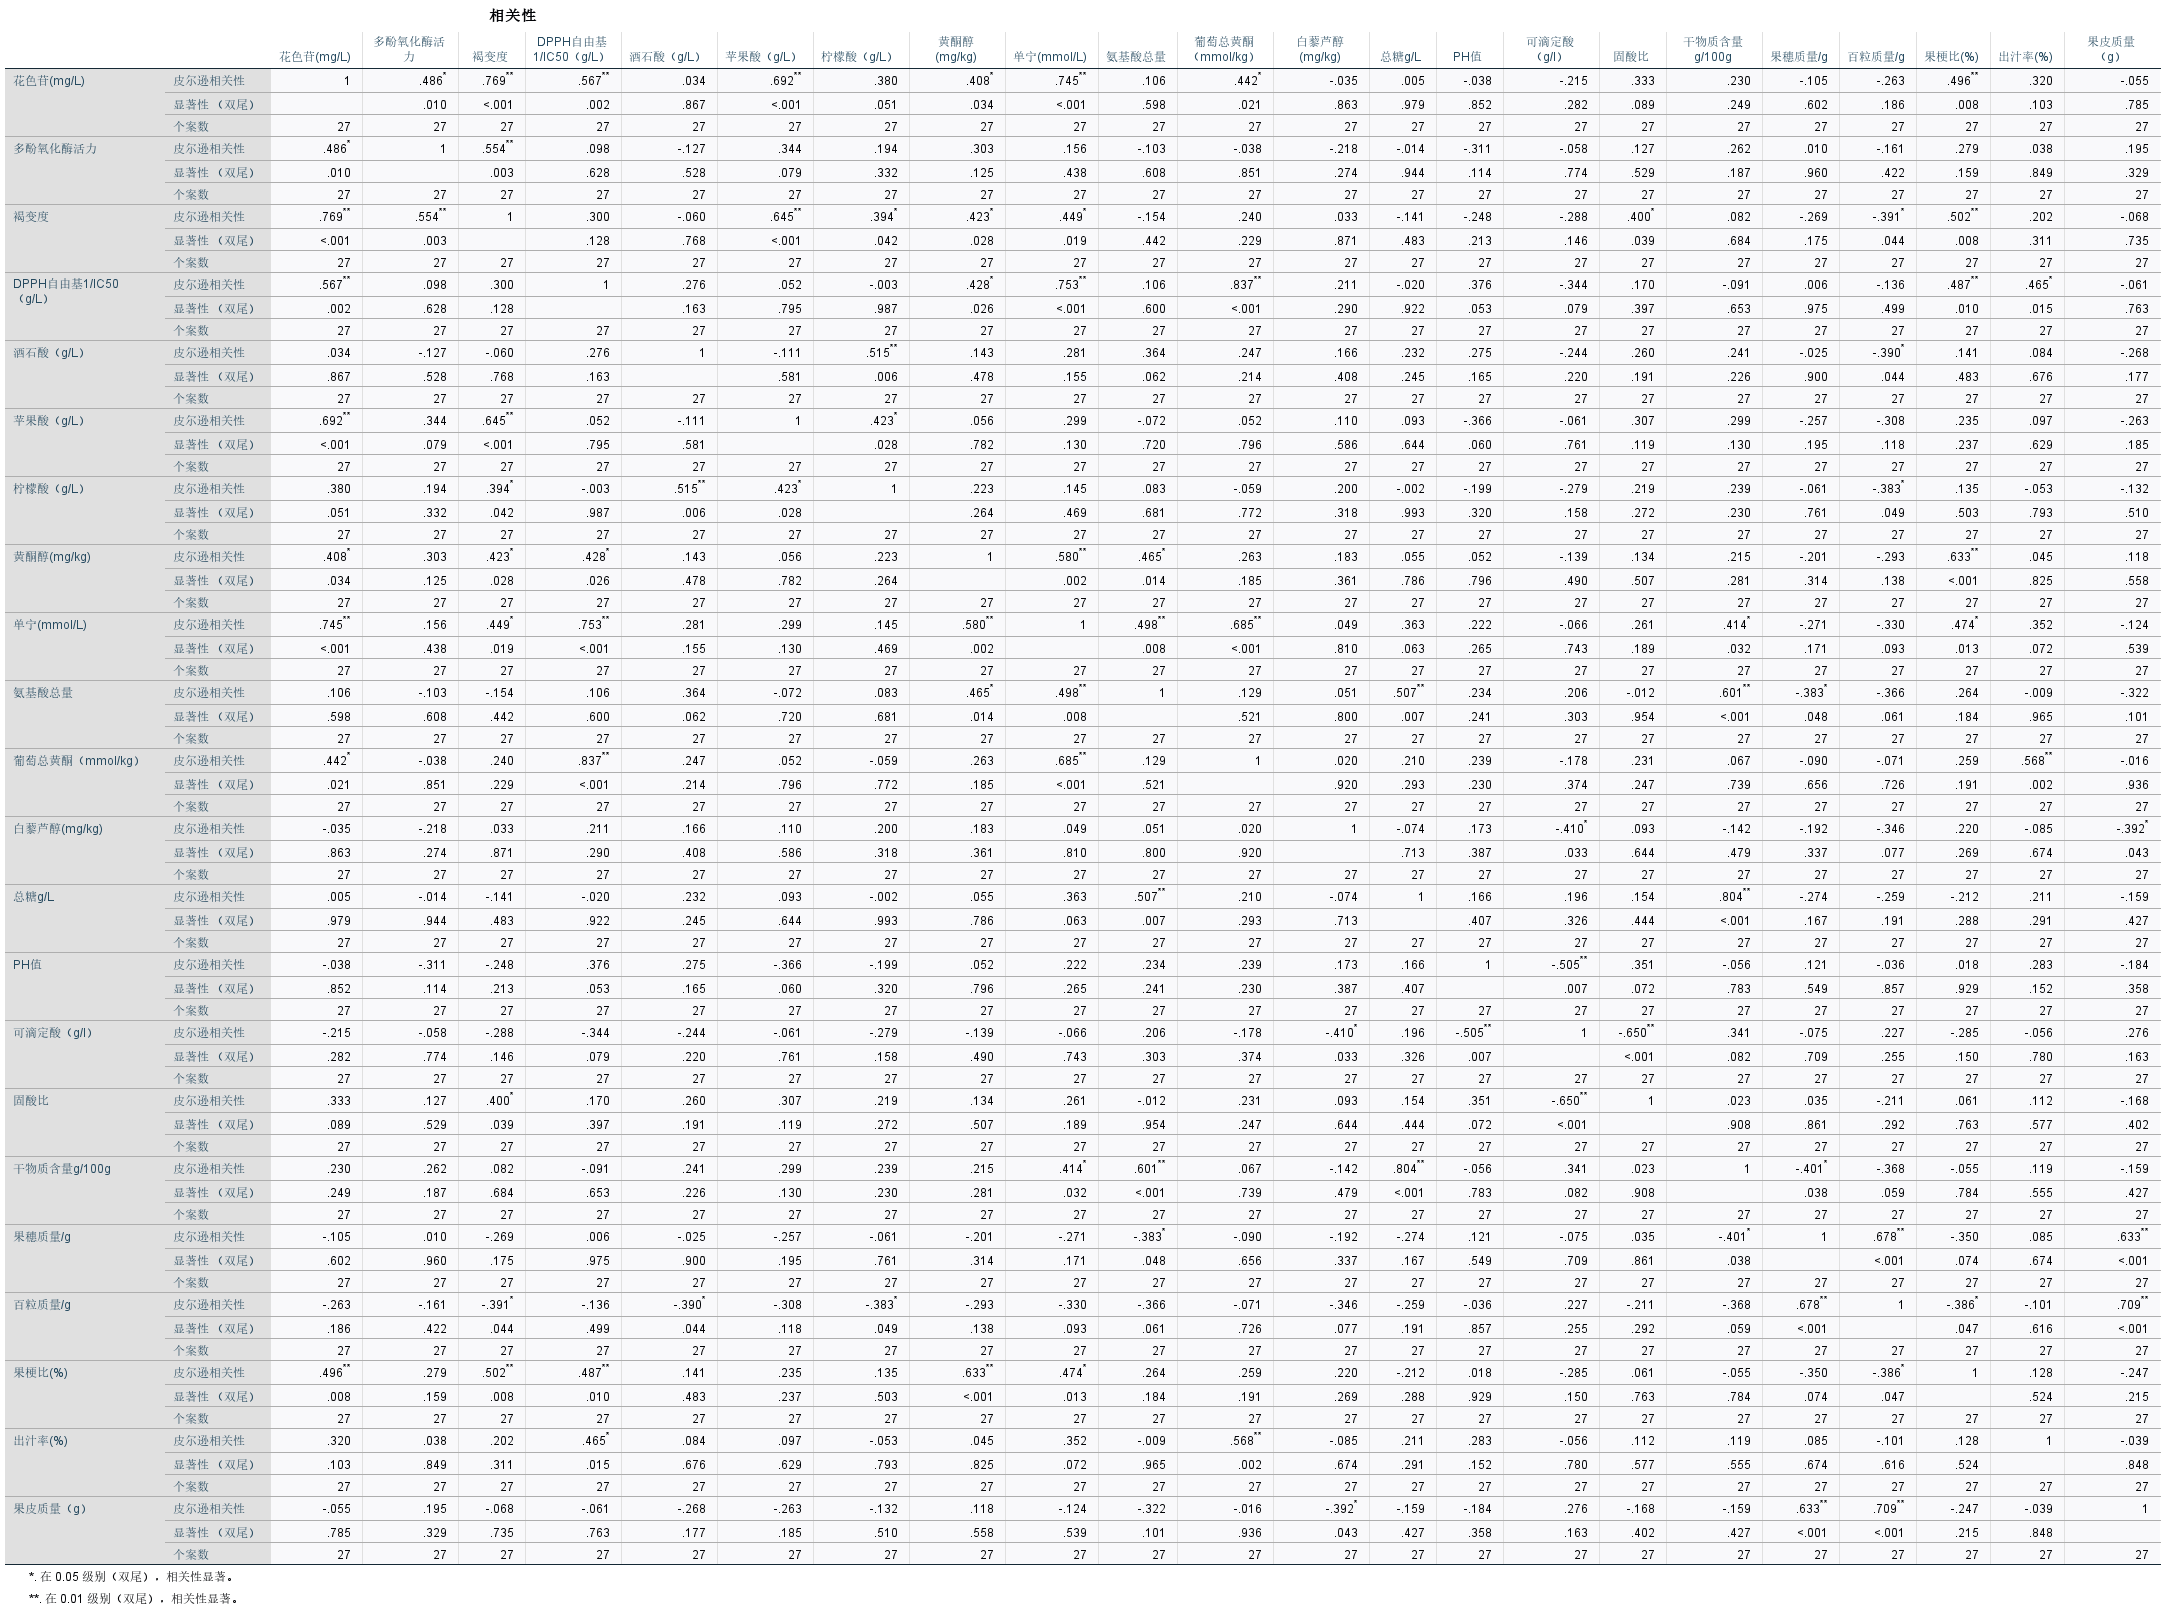
\includegraphics[width=0.9\textwidth]{img/花色苷相关性数据.png} % 图片相对位置
				\caption{花色苷相关性数据} % 图片标题 
				\label{fig:figure 1} % 图片标签
				\end{figure}

				\begin{figure}[H]\centering
				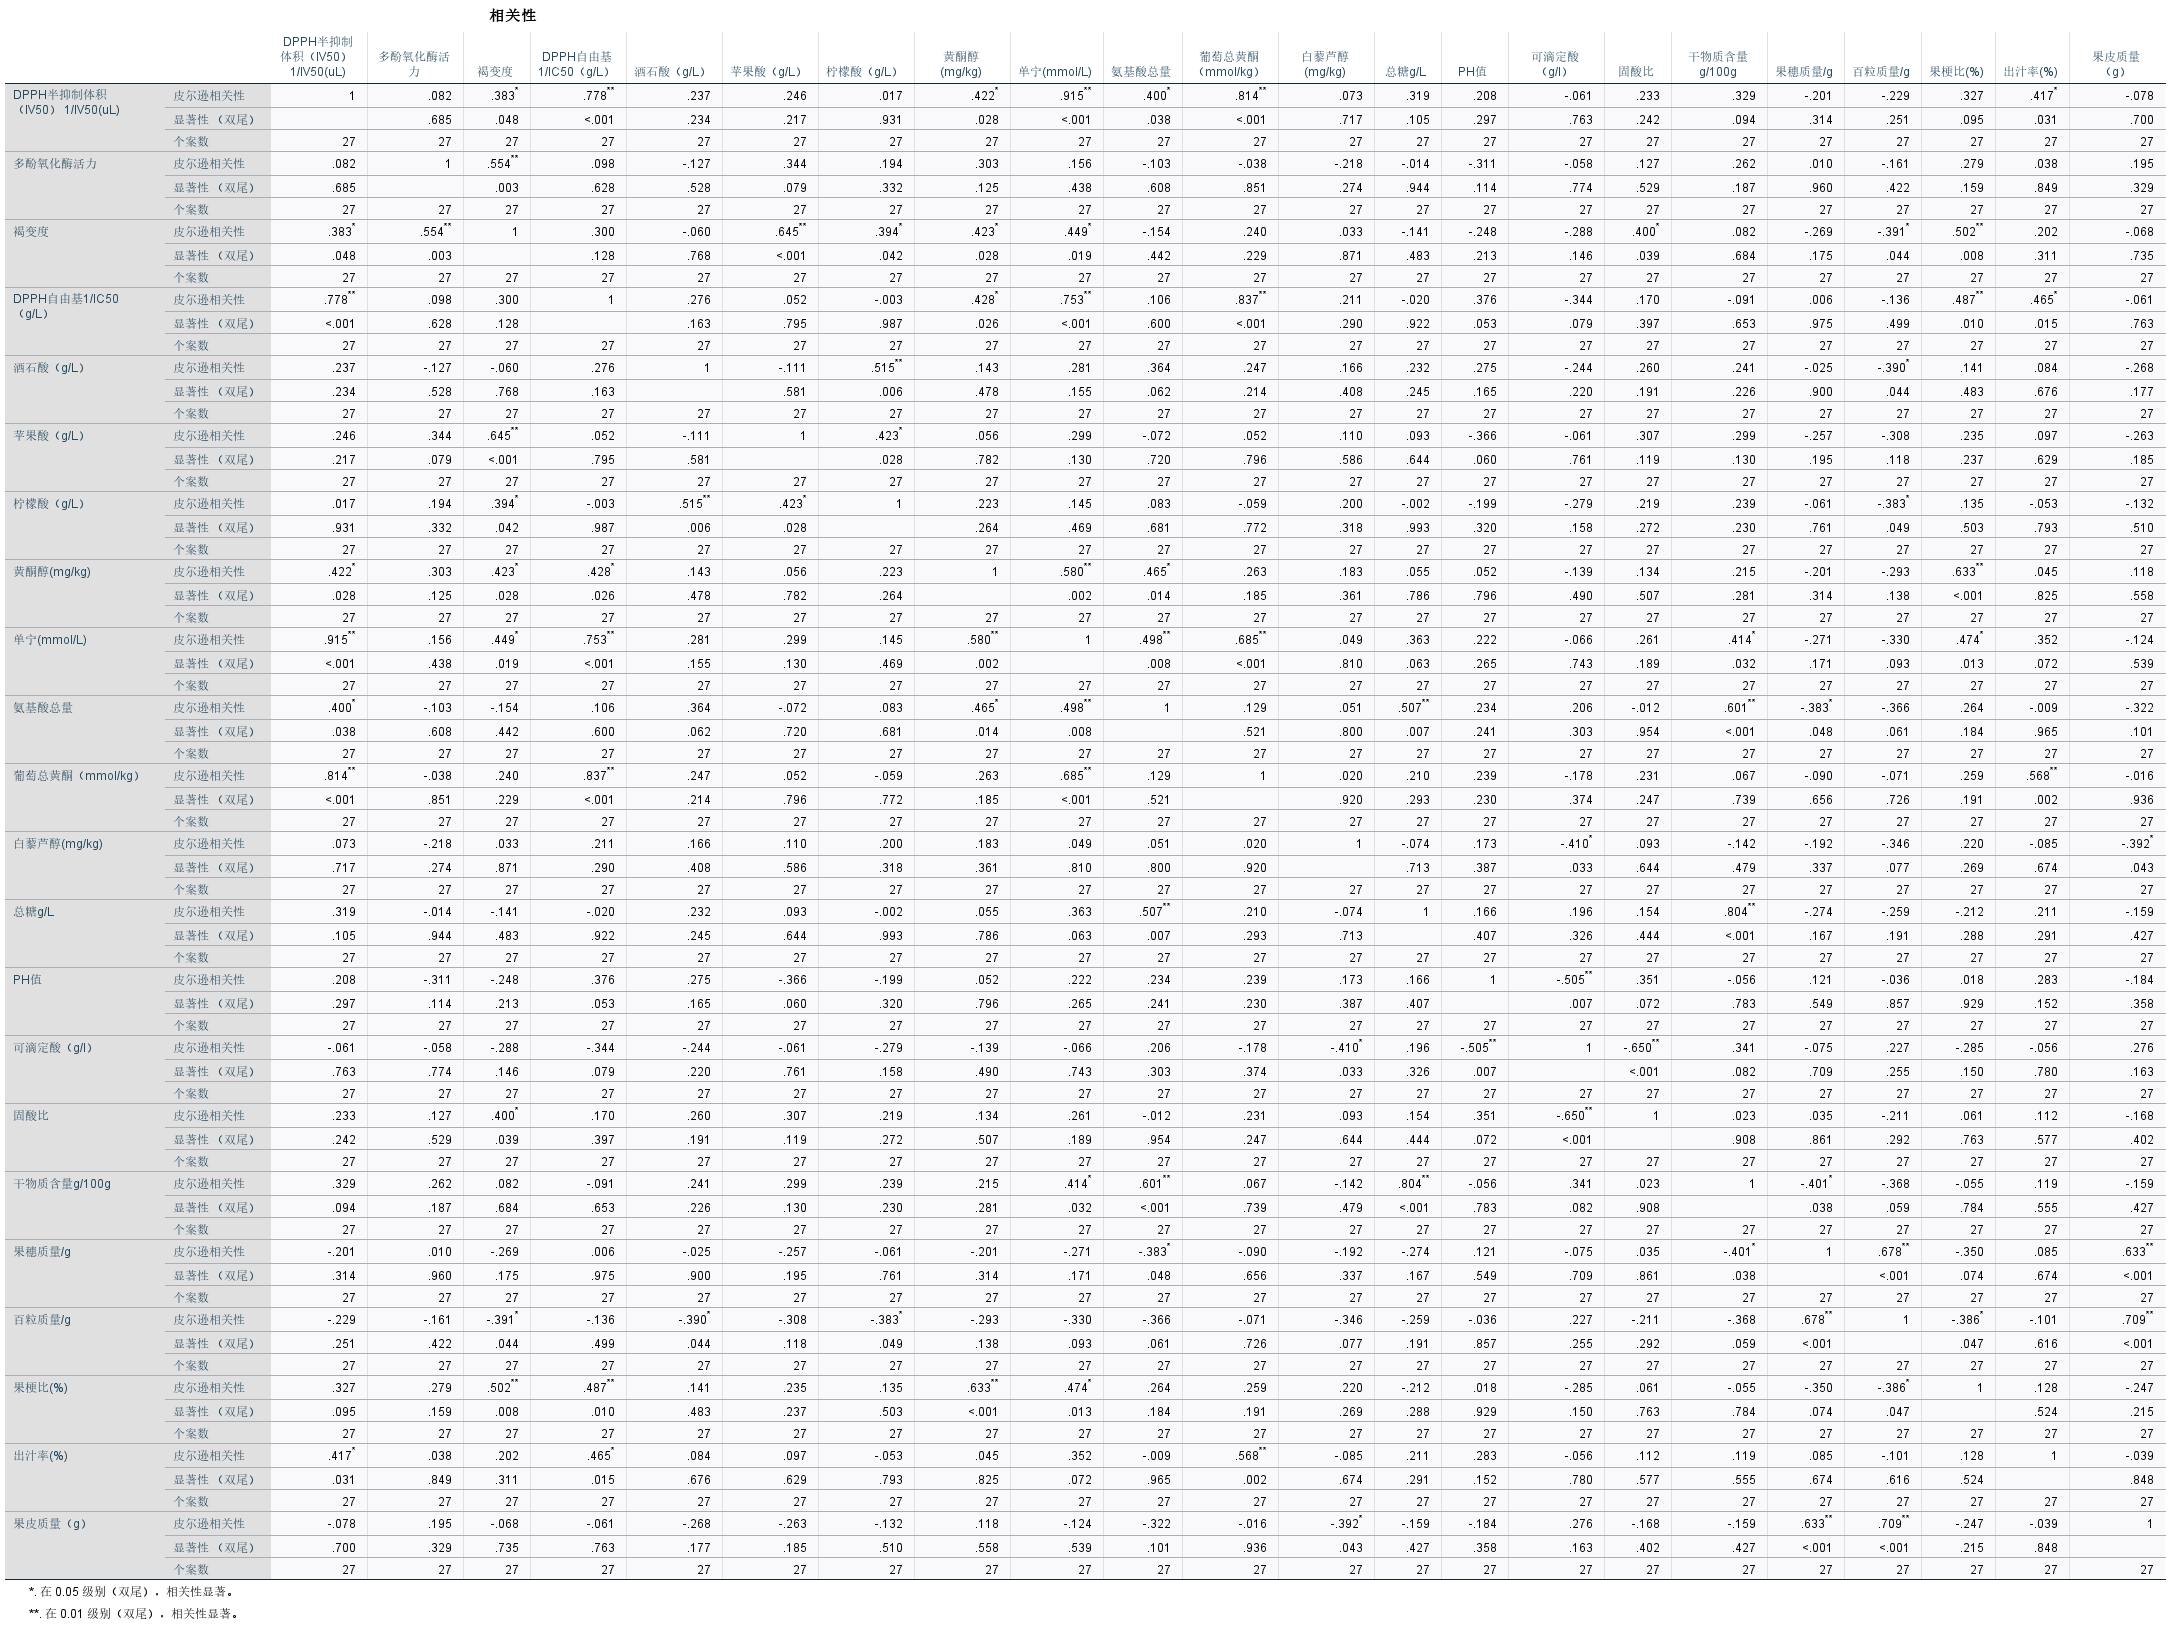
\includegraphics[width=0.9\textwidth]{img/DPPH半抑制体积相关性数据.png}
				\caption{DPPH半抑制体积相关性数据} % 图片标题 
				\label{fig:figure 2} % 图片标签
				\end{figure}
			

				\begin{figure}[H]\centering
					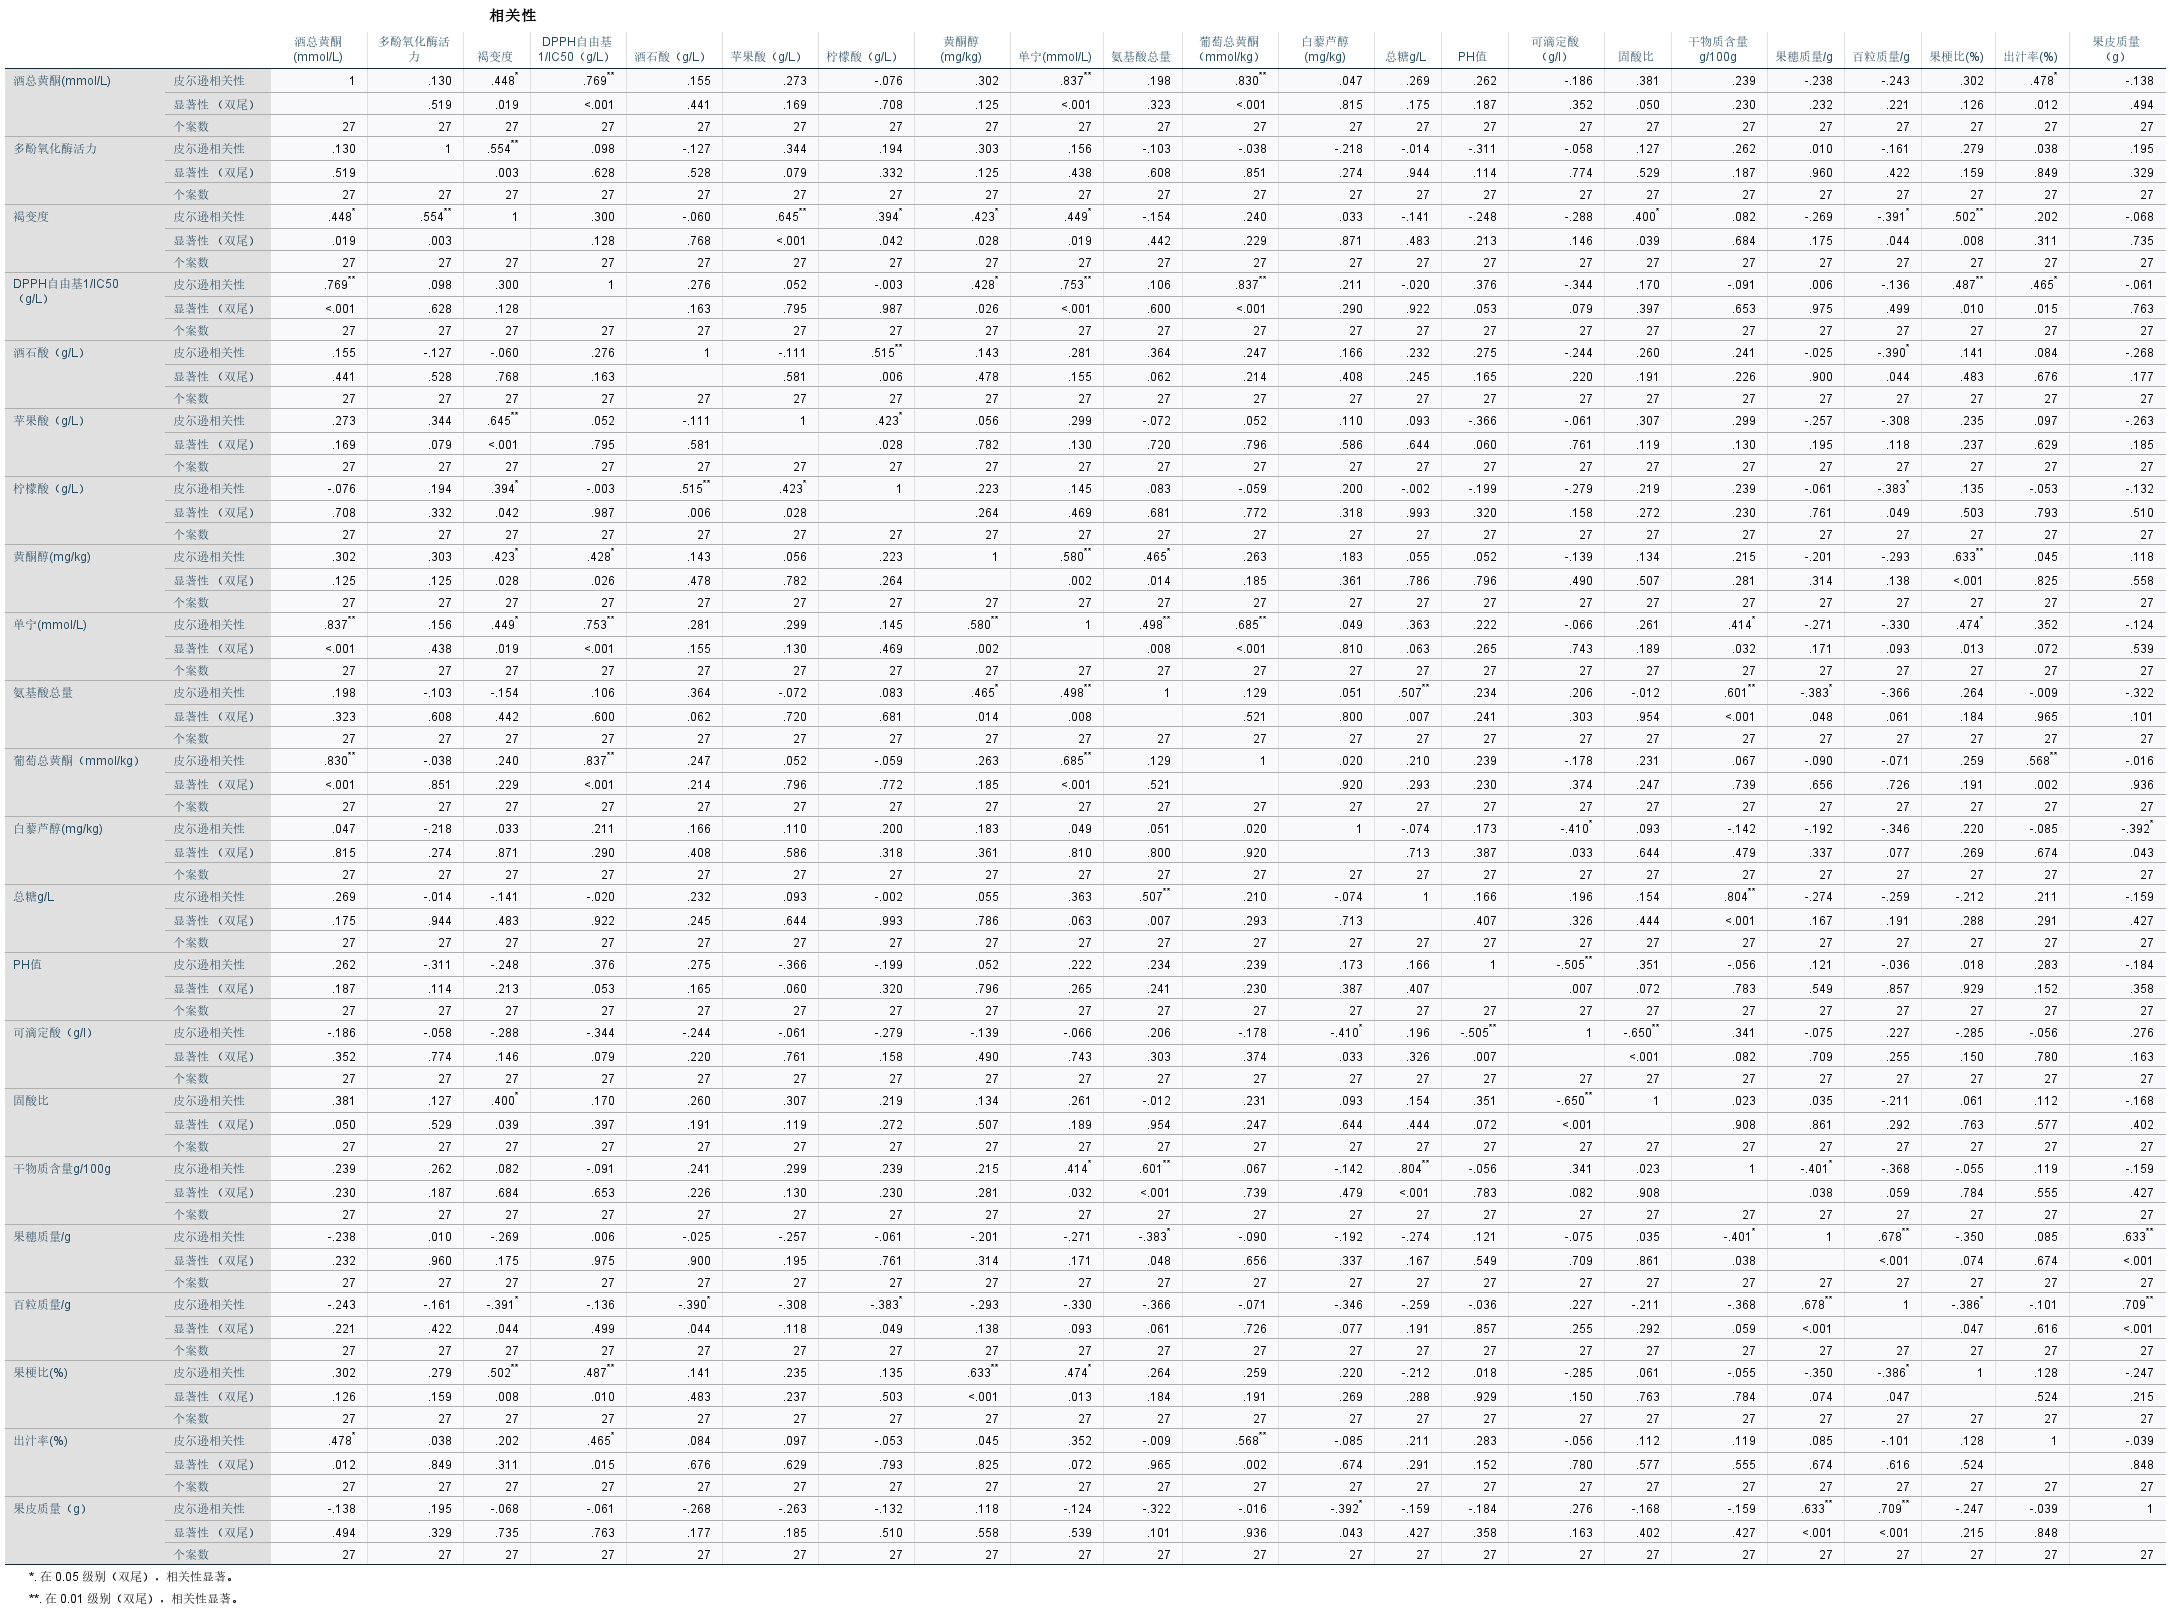
\includegraphics[width=0.9\textwidth]{img/酒总黄酮相关性数据.png} % 图片相对位置
					\caption{酒总黄酮相关性数据} % 图片标题 
					\label{fig:figure 3} % 图片标签
					\end{figure}

				\begin{figure}[H]\centering
					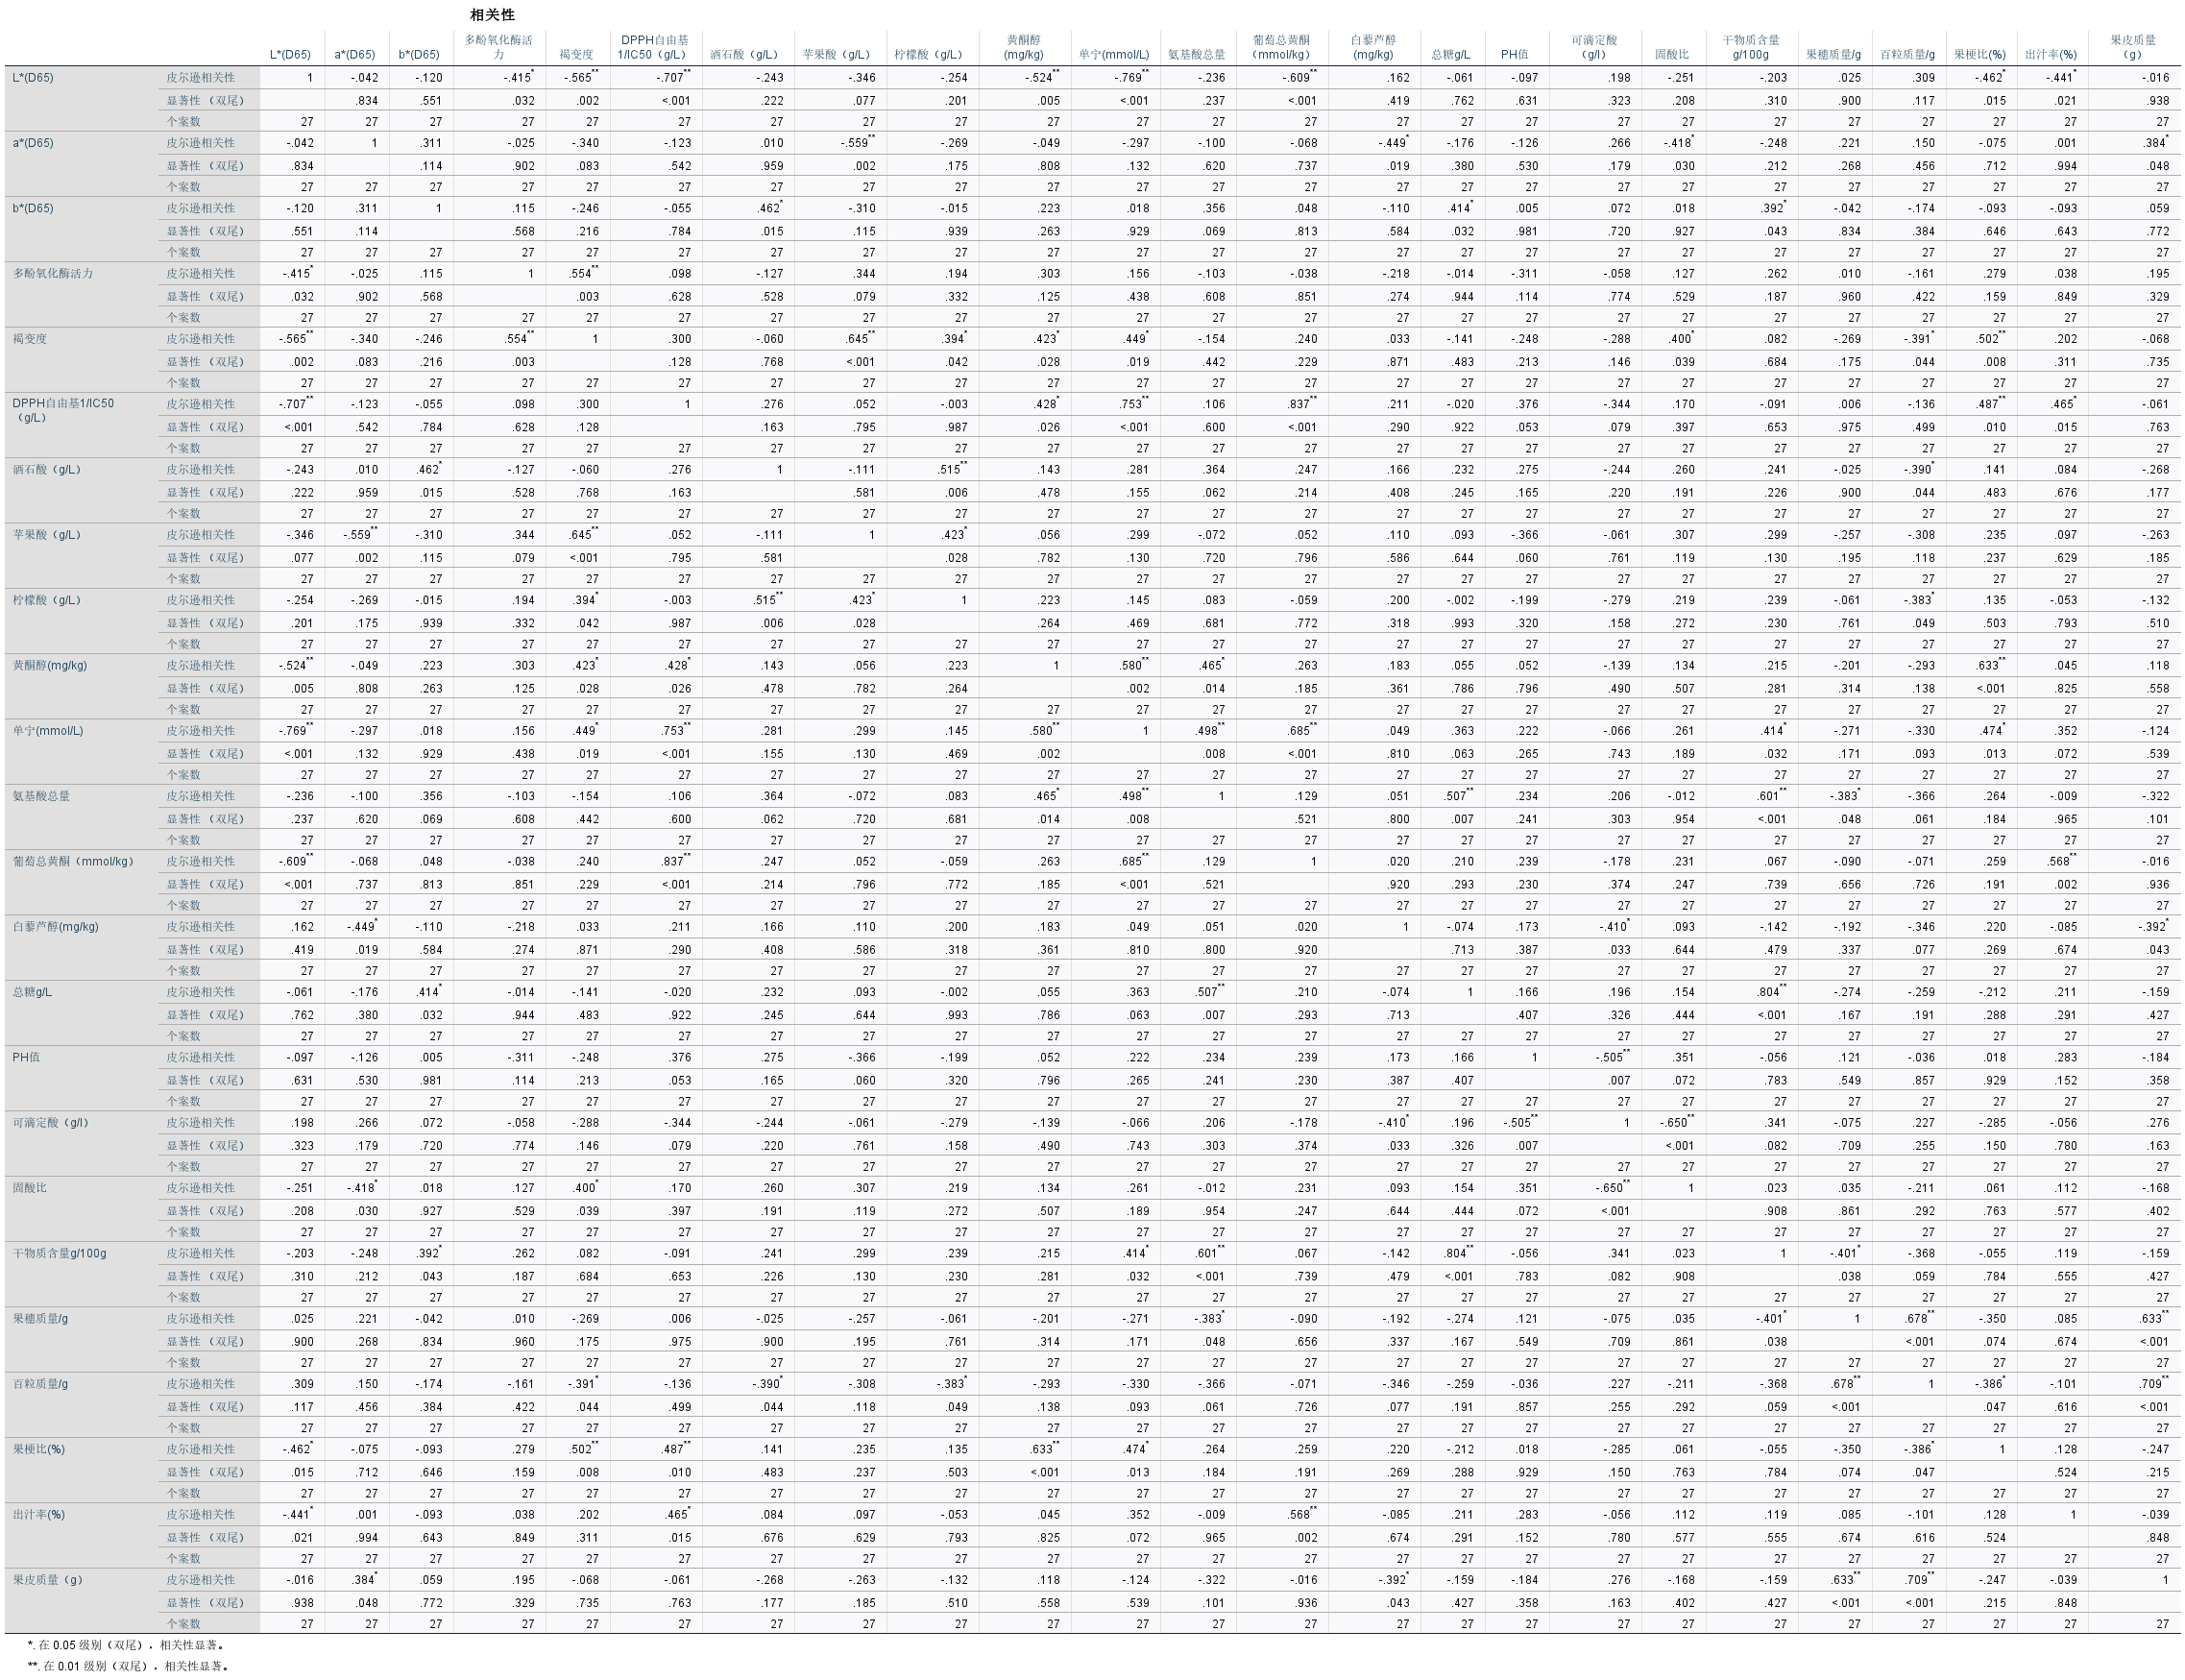
\includegraphics[width=0.9\textwidth]{img/色泽相关性数据.png} % 图片相对位置
					\caption{色泽相关性数据} % 图片标题 
					\label{fig:figure 4} % 图片标签
					\end{figure}

				\newpage

			\subsubsection{结果分析}
					对相关性分析的结果进行分析,其重点就是观察其pearson和双侧显著性的值,pearson相关系数的值大,则相关性高,同理观察算观测
					双侧显著性则是判断其值的范围,*p<0.05或者**p<0.01都证明其有较好的相关显著性。通过对结果进行分析,得出如下的一些较为明显
					的相关性结论:

					\begin{itemize}
						\item [{1)}]{花色苷的指标与褐变度、苹果酸、单宁、果梗比等数据的相关性较为显著}
						\item [2)]{DPPH半抑制体积与多酚氧化酶活力、DPPH自由基、单宁、葡萄总黄酮、白藜芦醇相关性高,与果皮质量和果穗质量等指标都成负相关}
						\item [3)]{酒总黄酮则跟DPPH自由基、单宁、葡萄总黄酮,白藜芦醇等指标相关性高}
						\item [4)]{色泽跟可滴定酸、果穗质量的略微相关,总体数据的相关性不大}
					\end{itemize}

					按照分析标准来分析,无论是相关性系数和显著程度都选取较为明显的那组数据来进行后面的关系分析。
					本小问中,在花色苷则这项数据所给出的相关性指标的相关性都较高,在多元回归中则考虑采取这项数据来进行拟合。

					\subsection{多元线性回归模型的求解}
					在建立模型则需要对模型进行拟合度检验,多元回归方程的显著性检验就是检验样本回归方程的变量的线性关系是否显著,
					需要根据样本来判断方程中的多个回归系数中至少有一个不等于0,主要是说明样本回归方程的显著性。
					检验的方法用方差分析,这时因变量的总体为回归平方和与误差平方和,即表示为:
						\begin{equation}
							L_xx = Q+U					
						\end{equation}
						其中该公式又可以表示为:
						\begin{equation}
							L_xx=\sum_{i=1}^{N}(y_i-\bar{y})^2
						\end{equation}
						\begin{equation}
							Q=\sum_{i=1}^{N}(y_i-\hat{y})^2
						\end{equation}
						\begin{equation}
							U=\sum_{i=1}^{N}(\hat{y_i}-\bar{y})^2
						\end{equation}
					
						对花色苷和其相关性较高的指标进行拟合,依据德宾沃森残差,离群值为3标准差进行模型拟合,来根据其R方及其
						德宾沃森残差来观察其拟合的契合度。
						另外进行单因素方差分析(ANOVA)来观测F检验对整个回归进行显著性检验,考虑的k个变量自变量是否有显著性线性关系
						F检测通过与F边界值来进行比对判断其水平显著性
						\[\left\{\begin{array}{llcl}
							F_0.05(k,n-k-1) \le F \le F_0.01(k,n-k-1){认为回归在0.05水平上显著} \\

							F_0.1(k,n-k-1) \le F \le F_0.05(k,n-k-1){认为回归在0.01水平上显著} \\

							F<F_0.1(k,n-k-1){则回归不显著} \\
						
					   \end{array} \right.\]
					   \subsubsection{单因素方差分析}
					   		对花色苷等多项相关性数据进行ANOVA分析,观察F检测值和显著性,通过三组不同数据的模型,对数据进行共线性诊断,依据
							VIF值来确定较为合理的自变量,来进行试验观察。
							得出如下的结果:				
							\begin{figure}[H]\centering
								
								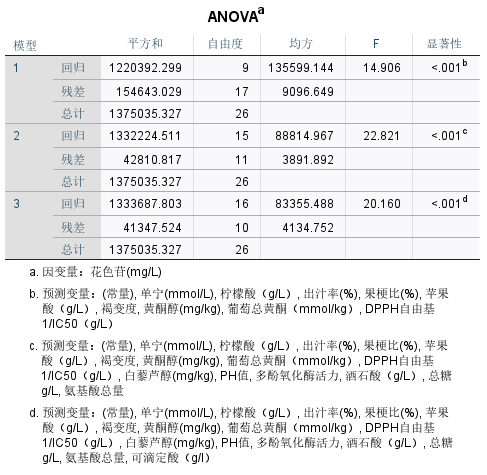
\includegraphics[width=0.52\textwidth,height=0.45\textwidth]{img/ANOVA.png} % 图片相对位置
								
								\caption{ANOVA} % 图片标题 	
								\label{fig:figure 5} % 图片标签
								\end{figure}

							分析观察三组回归的数据,发现三个模型的显著性都是<0.01,其F检测值分别为:14.906、22.821、20.160。根据该结果和显著性p值可以
							拒绝原假设,认为被解释变量个解释变量间存在显著的线性关系,可建立线性回归模型。
							
							如下为残差统计图:
							\begin{figure}[H]\centering
								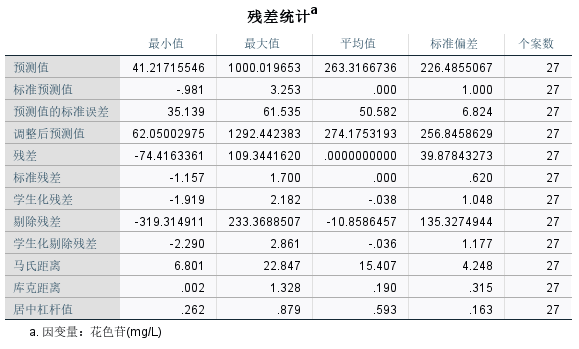
\includegraphics[width=0.52\textwidth,height=0.45\textwidth]{img/残差统计.png} % 图片相对位置
								\caption{残差统计} % 图片标题 	
								\label{fig:figure 6} % 图片标签
								\end{figure}
								在经过处理后的数据是比较合理的。

							\subsubsection{多元回归拟合}
							花色苷作为因变量,褐变度、苹果酸、单宁、果梗比、DPPH自由基、葡萄总黄酮、多酚氧化酶活力、总酚等相关性较为显著等数据作为自变量来进行多元回归拟合。
							在进行比对后发现并无需要严格剔除的数据,则进行多元线性回归变量筛选结果及系数的拟合求解。
							观察系数表和其显著性指标,通过${R^2}$来判断其回归拟合的契合度,往往${R^2}$越贴近于1,契合度越高。
							确定酿酒葡萄与葡萄酒理化指标的联系则将系数组合成回归方程即可。
							

								\begin{figure}[H]\centering
									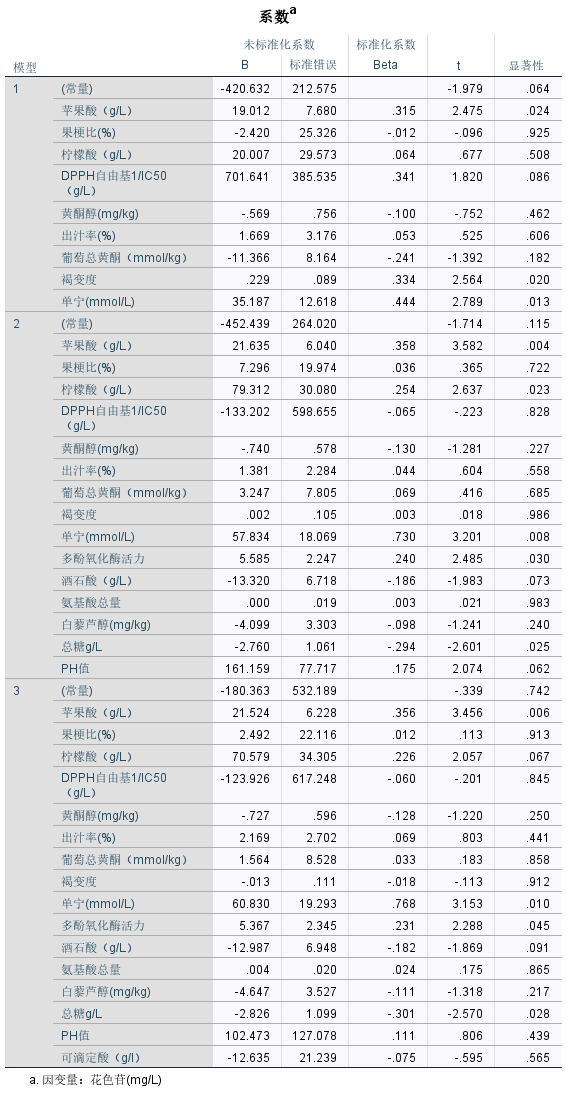
\includegraphics[width=0.8\textwidth,height=1.07\textwidth]{img/系数表.png} % 图片相对位置
									\caption{系数} % 图片标题 	
									\label{fig:figure 8} % 图片标签
									\end{figure}
								
								通过如下图表判断${R^2}$
							\begin{figure}[H]\centering
								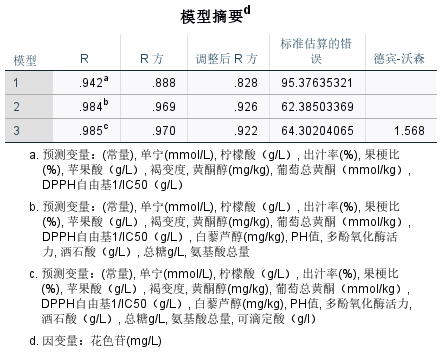
\includegraphics[width=0.52\textwidth,height=0.45\textwidth]{img/摘要表.png} % 图片相对位置
								\caption{摘要} % 图片标题 	
								\label{fig:figure 7} % 图片标签
								\end{figure}
								通过上述分析得出,三组数据的${R^2}$都相对趋近于1,具有较高的契合度。比对之后选择模型3的数据来进行方程的建立。
								由如下的系数表来得到系数关系。
								选取苹果酸、果梗比、柠檬酸、DPPH自由基、黄酮醇、出汁率.......等指标作为自变量${x_1,x_2,,,,,x_n}$构建如下方程:

								y=21.524{x_1}+2.49{x_2}+70.579{x_3}-123.926{x_4}-7.27{x_5}+2.169{x_6}+1.564{x_7}-0.013{x_8}+60.83{x_9}
								
								+5.367{x_{10}}-12.987{x_{11}}+0.004{x_{12}}-4.647{x_{13}}-2.826{x_{14}}+102.473{x_{15}}-12.635{x_{16}}-420.632
		
								其中$y$为因变量花色苷,${x_1,x_2,,,,,x_n}$则为自变量苹果酸、果梗比、柠檬酸、DPPH自由基、黄酮醇、出汁率.......
								通过该方程可以反映出葡萄酒的某些指标与酿酒葡萄理化指标之间的关系。
									

					



					

			







		   
		   

		%    \subsection{问题四的求解}

		   
		

		
		
		
		% \begin{figure}[!htbp]\centering
		% \includegraphics[width=0.9\textwidth]{img/} % 图片相对位置
		% \caption{各类人群转换流程图} % 图片标题 
		% \label{fig:figure 1} % 图片标签
		% \end{figure}	
		
		
		
	
		
% 		\vspace{4pt}
% 		\begin{itemize}
% 			\item [\textbf{a)}]关于易感者的变化,即疑似人群中未被感染的个体数减去未隔离的个体数。相应计算公式如下:\vspace{1ex}
% 				\begin{equation}
% 				\frac{dS(t)}{dt}=\kappa Y(t)-\rho S(t)N(t)
% 				\end{equation}
				
				
				
% 			\item[\textbf{b)}]关于感染者的变化,即为疑似人群中被确诊的个体数加未隔离患者个体数再减去退出者个体数,其中,退出个体数即已经治愈以及死亡的个体数之和。相应计算公式如下:\vspace{1ex}
% 				\begin{equation}
% 				\frac{dI(t)}{dt}=\omega N(t)+\lambda Y(t)-\xi I(t),
% 				\quad	\frac{dR(t)}{dt}=\xi I(t)
% 				\end{equation}	


				
% 			\item[\textbf{c)}]关于疑似者的变化,即为未隔离人群转为隔离人群(疑似者)的个体数减去隔离人群中被排除(确定未感染)的个体数,再减去隔离人群中被确诊的个体数。相应计算公式如下:\vspace{1ex}
% 				\begin{equation}
% 				\frac{dY(t)}{dt}=\theta N(t)S(t)-\kappa Y(t)-\lambda Y(t)
% 				\end{equation}	
				
				
				
% 			\item[\textbf{d)}]关于未隔离患者的变化,即为未隔离患者个体数减去被追踪到的未隔离患者的个体数。相应计算公式如下:\vspace{1ex}
% 				\begin{equation}
% 				\frac{dN(t)}{dt}=(1-\theta) N(t)S(t)-\omega N(t)
% 				\end{equation}	
				
% 		\end{itemize}
% 		\newpage
% 			\subsection{初值选取与参数确定}
% 		首先,我们选取了2月1日的疫情数据作为微分方程的初始值:

% 		\[\left\{\begin{array}{llcl}
% 		S(t_0)&=&140005\times10^4&\text{人},\\
% 		I(t_0)&=&14052 &\text{人},\\
% 		R(t_0)&=&130 &\text{人},\\
% 		Y(t_0)&=&4562 &\text{人},\\
% 		N(t_0)&=&6336 &\text{人},\\
% 		\end{array} \right.\]
		
% 		其次,通过查阅相关文献,我们确定了不同时期的各项参数:
% 		\[\left\{\begin{array}{lllll}
% 		\kappa_{1}&=0.06  ,&\kappa_{2}&=0.057\\
% 		\lambda_{1}&=0.44 ,&\lambda_{2}&=0.052\\
% 		\theta_{1}&=0.75  ,&\theta_{2}&=0.6\\
% 		\omega_{1}&=0.163 ,&\omega_{2}&=0.4\\
% 		\rho_{1}  &=0.45  ,&\rho_{2}&=0.45\\
% 		\xi_{1}   &=0.04  ,&\xi_{2}&=0.25\\
% 		\end{array}\right. \]

% 其中,下标1表示2-3月的参数,下标2表示3-5的参数		


% \vspace{1cm}	
% 			\subsection{模型求解}
% 		综上所述,可以得到模型:
% 		\[\left\{
% 		\begin{array}{ll}
% 		\displaystyle\frac{dS(t)}{dt}&=\kappa Y(t)-\rho S(t)N(t)        			 \vspace{1ex} \\
% 		\displaystyle\frac{dI(t)}{dt}&=\omega N(t)+\lambda Y(t)-\xi I(t) 		\vspace{1ex} \\
% 		\displaystyle\frac{dR(t)}{dt}&=\xi I(t)                         			 \vspace{1ex} \\
% 		\displaystyle\frac{dY(t)}{dt}&=\theta N(t)S(t)-\kappa Y(t)-\lambda Y(t)	\vspace{1ex} \\
% 		\displaystyle\frac{dN(t)}{dt}&=(1-\theta) N(t)S(t)-\omega N(t)			\vspace{1ex} \\
% 		\end{array}\right.\]\vspace{0.5cm}
% 		解得:
% 		\begin{equation}
% 		\text{感染总人数}\ \  \mathbf{I= a_1e^{-(\frac{t-b_1}{c_1})^2}+a_2e^{-(\frac{t-b_2}{c_2})^2}+a_3e^{-(\frac{t-b_3}{c_3})^2}   }
% 		\end{equation}\vspace{0.5cm}
% 		其中,各项参数为:
% 		\[\left\{\begin{array}{llllll}
% 		a_{1}&=9549 ,&a_{2}&=45380  ,&a_{3}&=9187\\
% 		b_{1}&=17.75 ,&b_{2}&=12.94 ,&b_{3}&=28.48\\
% 		c_{1}&=2.609 ,&c_{2}&=13.11 ,&c_{3}&=26.48\\
% 		\end{array}\right. \]
		
% 		\newpage
% 		\begin{figure}[!htbp]\centering
% 		\caption{微分方程组预测感染者与实际值对比}
% 		\includegraphics[width=1\textwidth]{img/figure 2} % 图片相对位置
% 		\label{fig:figure 2} % 图片标签
% 		\end{figure}
		
% 从图中可以我们可以发现我们的模型在整个时间跨度中具有实际情况符合程度极高的预测结果。另外,当我们只截取\ \textbf{五月($\mathrm{t}\in[90,120]$)}的数据进行对比,我们的模型仍然能比较好地预测感染人数的变化趋势。		
				
% 		\begin{figure}[!htbp]\centering
% 		\caption{微分方程、高斯拟合感染者与实际对比图}
% 		\includegraphics[width=1\textwidth]{img/figure 3}
% 		\label{fig:figure 3}
% 		\end{figure}
		
	
% 	\section{模型分析}
	
% 		\subsection{验证模型精确度}	
% 		计算预测数据与实际数据的相对误差,公式如下:
% 		\begin{equation}
% 		E=\frac{\displaystyle \sum_{i=1}^n\frac{|x_i-\hat{x}_i|}{x_i}}{\displaystyle n}=21.74\%
% 		\end{equation}
		
% 		考虑到中国人口基数大,疫情数据相对人口基数较小,该误差处于可接受的范围,又根据图中预测图像及实际图像可知,预测模型与实际情况基本吻合,说明该模型精确度较高。
		
% 		\subsection{误差分析}

% 			\begin{itemize}
% 				\item  在第10天左右,实际数值发生了激增,我们认为这是由于检测方法的优化和检测能力的提高,一天能检测的规模更大,因而产生了激增,这与我们的预测并不冲突。\vspace{-1.3ex}
% 				\item 疫情到达峰值之后的一段时间,实际数值下降的速率相比预测数值下降速率更慢,我们认为这是由于感染人数持续较多,增大了医院治疗的压力,对医疗物资的消耗较严重,因此下降速率更慢。
% 			\end{itemize}	
		
% 		\subsection{模型评价}
		
% 		\begin{itemize}
%    		\setlength{\parsep}{0ex} %段落间距
% 	    \setlength{\topsep}{2ex} %列表到上下文的垂直距离
%     	\setlength{\itemsep}{1ex} %条目间距
% 			\item \textbf{模型的优点}
% 			\begin{enumerate}[(1)]
% 			\item 预测范围较广,短中长期均可以预测
% 			\item 考虑到了现实中多种因素对疫情的干扰,更具实际意义
% 			\item 结合了中国此次抗疫所采取的高效有力的防控措施,区别于传统的传染病模型
% 			\end{enumerate}
% 			\item \textbf{模型的缺点}
% 			\begin{enumerate}[(1)]
% 			\item 没有考虑病毒的活性变化及突发事件
% 			\item 忽略了个体的体质等各方面的差异
% 			\end{enumerate}			
% 		\end{itemize}	
% 		\subsection{模型改进方向}
% 		\begin{itemize}
% 		\item 重新选取微分方程预测的初始值以及时间段
% 		\item 改变微分方程的参数,将其由常数变为随时间t变化的函数,以更好地拟合实际情况
% 		\end{itemize}
		
% \section{疫情防控建议}
% 		\begin{enumerate}[1)]
%  	\item 实施居家隔离、封城、公共领域限制等一系列持续地严防严控举措,进而降低疫情传播规模。
%   	\item 对疑似感染者集中快速隔离和诊断,进而缩减疫情扩散区域,阻碍疫情多点散花似扩散。
%   	\item 加强建设优质且全方位覆盖的公共卫生基础设施以及提高公共卫生治疗水平。
  
% 		\end{enumerate}		

\end{document}